\documentclass{swp1}
\usepackage[utf8]{inputenc}
\usepackage{amssymb}
\usepackage{url}


% Tabellen
\usepackage{tabularx}
\usepackage{supertabular}
\usepackage{booktabs}







\begin{document}

% \maketitle{Nummer}{Abgabedatum}{Tutor-Name}{Gruppennummer}
%           {Teilnehmer 1}{Teilnehmer 2}{Teilnehmer 3}
\maketitle{4}{13.07.2014}{Michaela Bunke}{ChronoX}
          {Tim Ellhoff}{Karsten Betjemann}{}
          
\section*{Aufgabe 1)}

\begin{figure}[h]
\centering{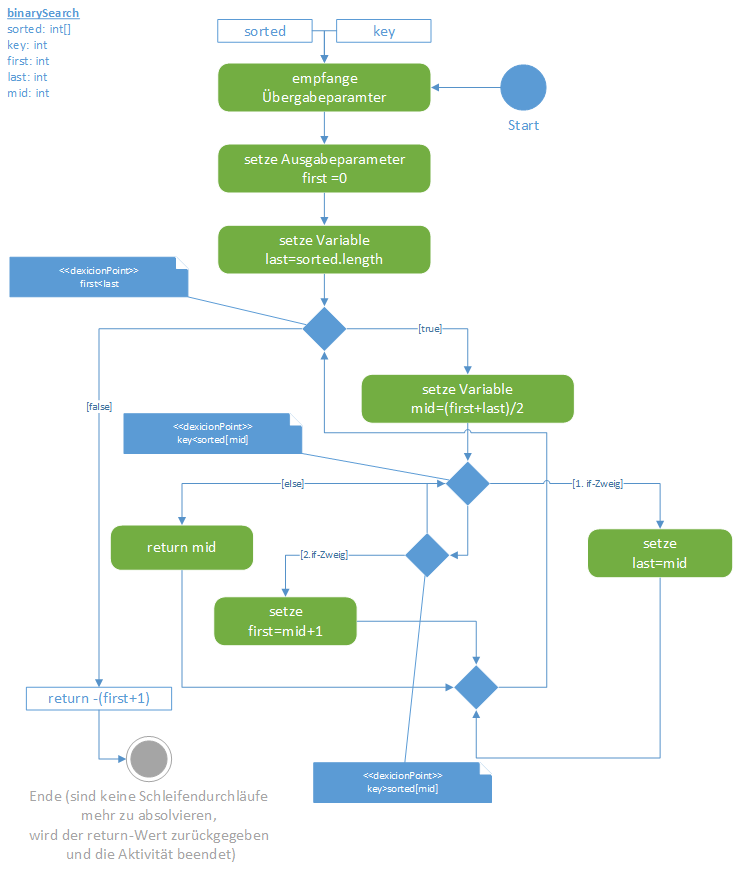
\includegraphics[width=13cm]{aufg1.png}}
\caption{Kontrollfluss der Java-Methode \texttt{binarySearch} in einem Aktivitätsdiagramm dargestellt}
\label{ab1}
\end{figure}


\section*{Aufgabe 2)}
\section*{Aufgabe 3)}
\section*{Aufgabe 4)}

Dargestellt ist der Ablauf in einem Online-Shop, visualisiert in einem Sequenzdiagramm. Dabei regelt die Klasse \texttt{ShoppingSession} die Shop-Sitzung und ist ebenso für die Darstellung des Shops zuständig. Die Klasse \texttt{Cart} stellt einen Einkaufswagen dar und die Klasse \texttt{ProductDB} repräsentiert den Zugriff auf die Produktdatenbank.

\textbf{Beschreibung des abgebildeten Vorgangs:}\\
Der Kunde ruft zunächst durch entsprechende Eingaben den Online-Shop auf. Es wird dabei eine Shop-Sitzung durch die Klasse \texttt{ShoppingSession} erstellt. Der Kunde sucht ein Notebook. Dazu gibt er in einem Suchfeld das Stichwort \glqq Notebook\grqq ein. Die \texttt{ShoppingSession} verarbeitet die Suchanfrage des Kunden und überprüft mit ihrer Methode \texttt{searchProducts} die Produktdatenbank \texttt{ProductDB} auf Treffer.\\
Die \texttt{ProductDB} liefert der \texttt{ShoppingSession} eine Liste mit Produkten zurück, die dem Kunden dann, wahrscheinlich in ansprechender Form (für die Darstellung ist auch die Klasse \texttt{ShoppingSession} zuständig) umgehend angezeigt wird.\\
der Kunde möchte sich Produktdetails von \textit{X123} anzeigen lassen. Die \texttt{ShoppingSession} ruft ihre Methode \texttt{getProductDetails} mit dem entsprechendem Parameter auf und fragt die Datenbank danach ab. \\
Die Datenbank liefert wiederum eine Liste mit Details zurück, die wieder in ansprechender Form dem Kunden von der \texttt{ShoppingSession} angezeigt werden.\\
Der Kunde entschließt sich dazu, das Gerät \texttt{X123} zu kaufen und legt es durch entsprechende Eingaben in den Warenkorb. Letzterer wird durch die Klasse \texttt{Cart} modelliert. Der Konstruktur der Klasse wird aufgerufen und mittels der \texttt{add}-Methode und dem entsprechendem Parameter wird das Gerät tatsächlich in den virtuellen Warenkorb bewegt, da die Methode \texttt{true} zurückliefert. Dies wird an die \texttt{ShoppingSession} weitergeleitet, die dann diese Information in verständlicher Form an den Kunden weiterleitet. \\
Zum Schluss überlegt es sich der Kunde doch noch mal anders und bricht seinen Einkauf ab, indem er durch entsprechende Eingaben (z.B. Löschen des Warenkorbs oder Ausloggen) der \texttt{ShoppingSession} den Abbruch mitteilt. Diese ruft die \texttt{clearProducts}-Methode auf und der entsprechende Teil der Datenbank wird geleert bzw. gelöscht. Schließlich liefert die Methode \texttt{true} zurück und die Aktion wurde erfolgreich abgebrochen. Der Warenkorb dürfte somit wieder leer sein.



\textbf{Äquivalentes Kommunikationsdiagramm:}\\


\end{document}

